
% This LaTeX was auto-generated from MATLAB code.
% To make changes, update the MATLAB code and republish this document.

\documentclass{article}
\usepackage{graphicx}
\usepackage{color}

\sloppy
\definecolor{lightgray}{gray}{0.5}
\setlength{\parindent}{0pt}

\begin{document}

    
    \begin{verbatim}
function secondTask
A = [0, 1; 0, -3]; % матрица на коефициенти
B = @(x)[0; myFunction(x)]; % свободни коефициенти
expA = expm(A); % матрична експонента

% начални условия
y0 = [0; 0];
% създаване на масив от времеви точки
t = linspace(0, 5, 100);
% създаване на масив за съхранение на резултатите
y = zeros(length(y0), length(t));

for i = 1:length(t)
    integrand = @(s) expm(A*(t(i)-s)) * B(s);
    y(:,i) = expA * y0 + integral(integrand, 0, t(i), 'ArrayValued', true);
end

figure(2),plot(t, y(1,:),t,y(2,:));
title('Графика на y по метода на матричната експонента');
xlabel('x');
ylabel('y');
legend('y1', 'y2', 'Location', 'northwest', 'Orientation', 'vertical');

end

function f = myFunction(x)
f = x*exp(-2*x);
end
\end{verbatim}

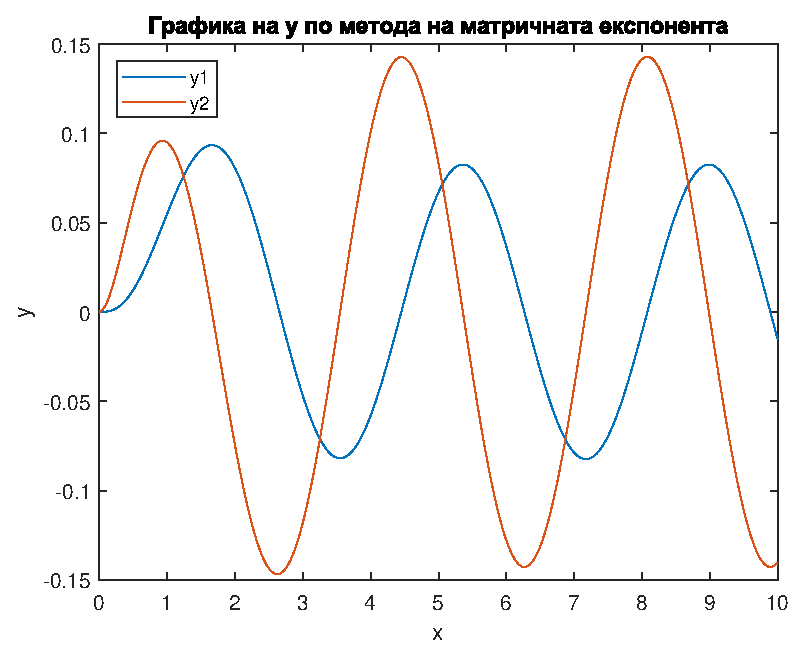
\includegraphics [width=4in]{secondTask_01.eps}



\end{document}

